% =====================================================================
% Two-page two-column summary report
% MSc Computational Finance, King's College London
% Huseyin Sarp Vulas  -  Supervisor: Dr Bart de Keijzer
% Figures: python scripts/make_figures.py  ->  docs/figures/*.dat
% Compile: pdflatex report_2page && pdflatex report_2page
% =====================================================================
\documentclass[10pt,a4paper,twocolumn]{article}

\usepackage[utf8]{inputenc}
\usepackage[T1]{fontenc}
\IfFileExists{lmodern.sty}{\usepackage{lmodern}}{}

\usepackage[margin=1.5cm,columnsep=0.6cm]{geometry}
\IfFileExists{lmodern.sty}{\usepackage{microtype}}{\usepackage[expansion=false]{microtype}}
\setlength{\parskip}{2pt}
\setlength{\parindent}{12pt}

\usepackage{amsmath,amssymb}
\usepackage{booktabs}
\usepackage{array}
\usepackage{graphicx}
\usepackage{xcolor}
\usepackage{caption}
\captionsetup{font=footnotesize,labelfont=bf,skip=3pt}

\usepackage{tikz}
\usepackage{pgfplots}
\pgfplotsset{compat=1.17}
\usetikzlibrary{positioning,arrows.meta,calc}

\usepackage[round,authoryear]{natbib}
\bibliographystyle{plainnat}
\usepackage[hidelinks]{hyperref}

\usepackage{titlesec}
\titleformat{\section}{\normalsize\bfseries}{\thesection}{0.5em}{}
\titlespacing{\section}{0pt}{5pt}{2pt}
\titleformat{\subsection}{\small\bfseries}{\thesubsection}{0.5em}{}
\titlespacing{\subsection}{0pt}{3pt}{1pt}

\newcommand{\prauc}{\mbox{PR-AUC}}
\newcommand{\rocauc}{\mbox{ROC-AUC}}
\definecolor{addgreen}{RGB}{27,120,55}
\definecolor{regblue}{RGB}{69,117,180}
\definecolor{crisisred}{RGB}{215,48,39}

% --- compact title ----------------------------------------------------
\title{\vspace{-1.2cm}\bfseries Dense Drawdown Supervision for Equity Crisis
Early Warning:\\ A Multi-Task Temporal Fusion Transformer and an Honest Test
of Regime Awareness}
\author{H\"useyin Sarp Vula\c{s}\quad\small Supervisor: Dr Bart de Keijzer\\
\small MSc Computational Finance, King's College London}
\date{\vspace{-0.4cm}}

\begin{document}
\maketitle
\thispagestyle{empty}\pagestyle{empty}

\begin{abstract}\small\noindent
Single-market equity crisis early-warning systems (EWS) are data-starved and
gradient-boosted trees usually win. Taking the Temporal Fusion Transformer
(TFT) as a backbone, we test, under a leak-free walk-forward protocol with a
63-day embargo and paired significance tests, whether \emph{regime awareness}
(a differentiable HMM regime module $+$ regime-conditioned attention bias)
helps. It does not: a fully regime-aware TFT is indistinguishable from a
vanilla TFT ($p{=}0.43$). What helps is a multi-task \emph{auxiliary
forward-drawdown head} $+$ \emph{focal loss} (``AF''): it beats vanilla TFT
single-market (macro $\prauc$ $0.483$ vs.\ $0.458$, $p{=}0.027$) with far
better calibration, and, scaled to a nine-market panel ($\approx$110
episodes), beats XGBoost ($\prauc$ $0.399$ vs.\ $0.373$). Dense supervision
beats architectural ornament; protocol beats headline.
\end{abstract}

% ===== full-width figures (span both columns) ========================
\begin{figure*}[t]
\centering
\begin{tikzpicture}
\begin{axis}[
  width=0.92\textwidth, height=4.3cm,
  ymode=log, log basis y=10,
  xlabel={year}, ylabel={S\&P 500 (log)},
  xmin=2000, xmax=2026.5, ymin=600, ymax=8000,
  tick label style={font=\scriptsize}, label style={font=\footnotesize},
  enlargelimits=false, clip=true,
]
\fill[crisisred!18] (axis cs:2007.75,600) rectangle (axis cs:2009.45,8000);
\fill[crisisred!18] (axis cs:2011.33,600) rectangle (axis cs:2012.42,8000);
\fill[crisisred!18] (axis cs:2015.58,600) rectangle (axis cs:2016.10,8000);
\fill[crisisred!18] (axis cs:2018.75,600) rectangle (axis cs:2018.99,8000);
\fill[crisisred!18] (axis cs:2020.13,600) rectangle (axis cs:2020.33,8000);
\fill[crisisred!18] (axis cs:2022.00,600) rectangle (axis cs:2022.83,8000);
\addplot[regblue,very thick,mark=none] table[x=t,y=close] {figures/spx_timeline.dat};
\end{axis}
\end{tikzpicture}
\caption{S\&P~500 (log), 2000--2026, with the six crisis episodes used as
walk-forward test folds shaded: GFC, Eurozone, China-2015, Q4-2018, COVID,
2022 bear. Each fold trains on the expanding prior history (with a 63-day
embargo) and tests on the shaded crisis.}
\label{fig:timeline}
\end{figure*}

\begin{figure*}[t]
\centering
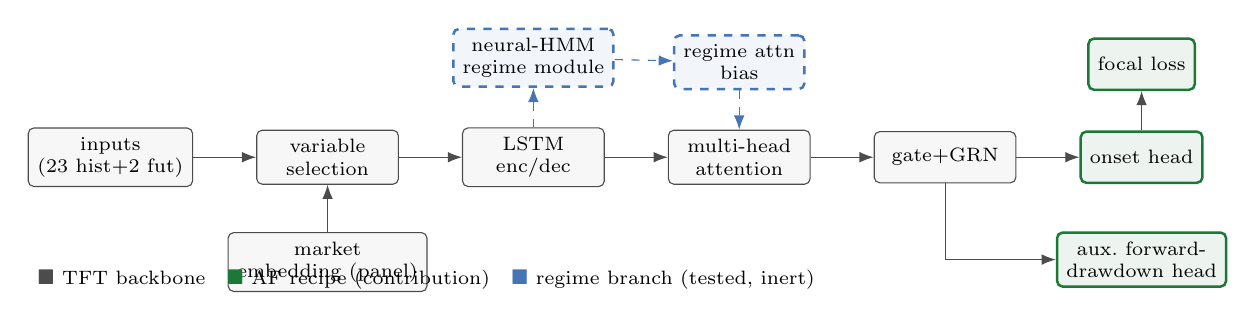
\begin{tikzpicture}[
  font=\scriptsize,
  box/.style={draw=black!70,rounded corners=2pt,minimum height=6.5mm,minimum width=18mm,align=center,fill=black!3},
  add/.style={draw=addgreen,line width=0.9pt,rounded corners=2pt,minimum height=6.5mm,align=center,fill=addgreen!8},
  reg/.style={draw=regblue,dashed,line width=0.9pt,rounded corners=2pt,minimum height=6.5mm,align=center,fill=regblue!7},
  ar/.style={-{Latex[length=1.8mm]},black!70},
  node distance=5mm and 8mm,
]
\node[box] (inp) {inputs\\(23 hist+2 fut)};
\node[box,right=of inp] (vsn) {variable\\selection};
\node[box,right=of vsn] (lstm) {LSTM\\enc/dec};
\node[box,right=of lstm] (attn) {multi-head\\attention};
\node[box,right=of attn] (grn) {gate+GRN};
\node[add,right=of grn] (head) {onset head};
\draw[ar] (inp)--(vsn); \draw[ar] (vsn)--(lstm); \draw[ar] (lstm)--(attn);
\draw[ar] (attn)--(grn); \draw[ar] (grn)--(head);
\node[box,below=6mm of vsn] (stat) {market\\embedding (panel)};
\draw[ar] (stat)--(vsn);
\node[add,below=6mm of head] (aux) {aux.\ forward-\\drawdown head};
\draw[ar] (grn)|-(aux);
\node[add,above=5mm of head] (focal) {focal loss};
\draw[ar] (head)--(focal);
\node[reg,above=5mm of lstm] (hmm) {neural-HMM\\regime module};
\node[reg,above=5mm of attn] (bias) {regime attn\\bias};
\draw[ar,regblue,dashed] (lstm)--(hmm); \draw[ar,regblue,dashed] (hmm)--(bias);
\draw[ar,regblue,dashed] (bias)--(attn);
\node[anchor=west,font=\scriptsize] at ($(inp.west)+(0,-1.55)$)
 {\textcolor{black!70}{$\blacksquare$}~TFT backbone \;
  \textcolor{addgreen}{$\blacksquare$}~AF recipe (contribution) \;
  \textcolor{regblue}{$\blacksquare$}~regime branch (tested, inert)};
\end{tikzpicture}
\caption{Model. Black: TFT backbone \citep{lim2021tft}. Green: the AF recipe
(multi-task auxiliary forward-drawdown head $+$ focal loss), the contribution.
Blue/dashed: the regime module and regime-conditioned attention bias,
implemented and ablated but found inert.}
\label{fig:arch}
\end{figure*}

% ===== body ==========================================================
\section{Problem and approach}
A reliable early-warning system (EWS) for equity crises is of direct value to
risk managers and allocators \citep{kaminsky1999leading}. We predict crisis
\emph{onset} within a forward quarter $[t{+}1,t{+}63]$. The literature reports
that on single markets gradient-boosted trees match or beat neural sequence
models \citep{bluwstein2023credit,holopainen2017toward}; this is a property of
the \emph{formulation} (few episodes), not a law. We take the TFT
\citep{lim2021tft} as backbone (Fig.~\ref{fig:arch}) and ask two questions:
does a crisis-specific inductive bias --- \emph{regime awareness} --- help, and
if not, what does?

\textbf{Contributions.} (i) A leak-free evaluation that makes an earlier
random-holdout ``win'' reverse. (ii) A powered, honest test showing the regime
machinery is \emph{inert}. (iii) The AF recipe: dense drawdown supervision $+$
focal loss, which significantly and transferably improves on vanilla TFT.

\section{Data and labelling}
Daily Bloomberg data, 2000--2026: the S\&P~500 (single-market study) and a
nine-index panel (SPX, NDX, RTY, SX5E, SXXP, UKX, MCX, MXEF, MXWO; $61{,}996$
market-days, $\approx$110 crisis episodes vs.\ $\sim$5 on the S\&P~500 alone).
Inputs are a 252-day window of 23 historical features (multi-horizon returns,
realised vol, drawdown, Hurst, Amihud illiquidity, VIX, credit/TED spreads,
DXY, gold, MOVE, \dots) plus two known-future calendar features. The dataset
has \emph{no} static numerics, so TFT's static pathway activates only in the
panel, via a learned market embedding.

Crisis $=$ drawdown $|D_t|\ge\tau$ from the trailing 252-day peak; onset $=$
first crisis day after $\ge$20 calm days; target $y_t=\mathbf{1}\{$onset in
$[t{+}1,t{+}63]\}$. We choose $\tau{=}10\%$ from the empirical drawdown
distribution (mean $6.6\%$, s.d.\ $9.0\%$): $5\%$ is below the mean
($-0.18\sigma$, noise), $20\%$ is clean ($+1.49\sigma$) but yields $\sim$5
episodes; dd10 ($+0.38\sigma$, $23.6\%$ of days) is the defensible operating
point for a market-stress EWS.

\section{Method}
\textbf{Leak-free protocol.} Crisis-anchored walk-forward folds
(Fig.~\ref{fig:timeline}); a 63-day embargo purges the label-horizon rows at
each boundary \citep{lopezdeprado2018}; train/val/test are windowed
independently (strictly post-split); the scaler is train-only. Primary metric
$\prauc$ (read against prevalence \citep{saito2015prc}); also $\rocauc$, Brier,
Platt calibration; 30 seeds; paired Wilcoxon tests.

\textbf{The AF recipe.} Two changes to the \emph{learning problem}, not the
topology: a multi-task linear head regressing the continuous forward drawdown
(a dense signal present every day, unlike the sparse onset label), and focal
loss \citep{lin2017focal} on the classifier. With predicted probability $p$,
label $y$, predicted/target drawdown $\hat d,d$:
\begin{equation}\small
\mathcal{L}= -w_{+}y(1{-}p)^{\gamma}\log p-(1{-}y)p^{\gamma}\log(1{-}p)
+\lambda(\hat d-d)^2,
\end{equation}
with $\gamma{=}2$, $\lambda{=}0.5$, $w_{+}$ near the inverse prevalence.
``AFv2'' is AF with panel-matched capacity (hidden 128, 60 epochs, lr
$5\!\times\!10^{-4}$, per-market norm).

\section{Results}
\textbf{Backbone.} On clean splits, vanilla TFT ($0.515$) $>$ LSTM ($0.397$)
$>$ XGBoost ($0.320$) macro $\prauc$ --- the earlier ``LSTM wins'' was a
leakage artifact.

\textbf{Regime awareness is inert.} Factorially ablated, no component helps;
the full RA-TFT ties vanilla (Table~\ref{tab:sm}; $p{=}0.43$, 30 seeds, 6
folds). Adding seeds cannot fix this --- power is bounded by the number of
independent crisis \emph{episodes}, not seeds.

\textbf{The AF recipe wins.} AF beats vanilla TFT on every metric and is the
\emph{first} configuration to do so significantly on clean splits
(Table~\ref{tab:sm}, $p{=}0.027$); its calibration edge (Brier $0.270$ vs.\
$0.318$) is the clearest practical gain. The improvement concentrates in
severe regime-shift crises (COVID $+0.16$, China $+0.04$ $\prauc$) and is
neutral on mild corrections --- it helps most when it matters most.

\textbf{Panel.} With capacity matched to the larger data, AFv2 beats XGBoost
(Table~\ref{tab:panel}): $\prauc$ $0.399$ vs.\ $0.373$, $\rocauc$ $0.609$ vs.\
$0.585$. The regime module is inert again ($p{=}0.95$, a fifth confirmation);
the lever is capacity$+$epochs$+$loss, not per-market norm ($p{=}0.46$). The
same AFv2 config transfers back to the single market without loss --- one
unified recipe.

\begin{table}[t]
\centering\footnotesize
\caption{Single-market, 6 folds, $\approx$30 seeds. Macro $\prauc$ (raw/Platt),
Brier$\downarrow$. AF vs.\ vanilla $p{=}0.027$; RA-TFT vs.\ vanilla $p{=}0.43$.}
\label{tab:sm}
\begin{tabular}{lcccc}
\toprule
Model & raw $\prauc$ & Platt $\prauc$ & Brier & Platt Brier \\
\midrule
Vanilla TFT (M0)  & 0.458 & 0.545 & 0.318 & 0.285 \\
Full RA-TFT (M4)  & 0.460 & 0.623 & 0.305 & 0.270 \\
\textbf{AF (aux+focal)} & \textbf{0.483} & \textbf{0.656} & \textbf{0.270} & \textbf{0.239} \\
\bottomrule
\end{tabular}
\end{table}

\begin{table}[t]
\centering\footnotesize
\caption{Nine-market panel, pooled test (2019--2026), prevalence $0.300$.
AFv2 vs.\ vanilla$+$norm $p{=}0.039$.}
\label{tab:panel}
\begin{tabular}{lccc}
\toprule
Model & raw $\prauc$ & $\rocauc$ & Brier \\
\midrule
\textbf{AFv2 (tuned recipe)} & \textbf{0.399} & \textbf{0.609} & \textbf{0.269} \\
M0 $+$ per-market norm       & 0.377 & 0.597 & 0.347 \\
XGBoost                      & 0.373 & 0.585 & 0.273 \\
Vanilla TFT (M0)             & 0.343 & 0.552 & 0.368 \\
LSTM                         & 0.297 & 0.490 & 0.478 \\
\bottomrule
\end{tabular}
\end{table}

\section{Conclusion and future work}
A well-motivated crisis-specific inductive bias (regime awareness) does not
survive a powered, leak-free test, while a simple change to the learning
problem --- dense drawdown supervision $+$ focal loss --- does, transferably,
across single-market and panel settings, beating XGBoost on the panel. Future
work: more crisis episodes (the binding constraint) via a wider panel;
instrumented evaluation for reliability diagrams and block-bootstrap CIs; and
auxiliary-task design (multi-horizon / quantile drawdown heads).

\vspace{-2pt}
{\footnotesize
\bibliographystyle{plainnat}
\begin{thebibliography}{9}\setlength{\itemsep}{0pt}\small
\bibitem[Bluwstein et al.(2023)]{bluwstein2023credit} Bluwstein, K.\ et al.\ (2023). Credit growth, the yield curve and financial crisis prediction. \emph{J.\ Int.\ Econ.}, 145:103773.
\bibitem[Holopainen \& Sarlin(2017)]{holopainen2017toward} Holopainen, M.\ \& Sarlin, P.\ (2017). Toward robust early-warning models. \emph{Quant.\ Finance}, 17(12):1933--1963.
\bibitem[Kaminsky \& Reinhart(1999)]{kaminsky1999leading} Kaminsky, G.\ \& Reinhart, C.\ (1999). The twin crises. \emph{Amer.\ Econ.\ Rev.}, 89(3):473--500.
\bibitem[Lim et al.(2021)]{lim2021tft} Lim, B.\ et al.\ (2021). Temporal Fusion Transformers. \emph{Int.\ J.\ Forecast.}, 37(4):1748--1764.
\bibitem[Lin et al.(2017)]{lin2017focal} Lin, T.-Y.\ et al.\ (2017). Focal loss for dense object detection. \emph{ICCV}, 2980--2988.
\bibitem[L\'opez de Prado(2018)]{lopezdeprado2018} L\'opez de Prado, M.\ (2018). \emph{Advances in Financial Machine Learning}. Wiley.
\bibitem[Saito \& Rehmsmeier(2015)]{saito2015prc} Saito, T.\ \& Rehmsmeier, M.\ (2015). The precision-recall plot\dots \emph{PLOS ONE}, 10(3):e0118432.
\end{thebibliography}}

\end{document}
